\documentclass[./standalone.tex]{subfiles}
%\documentclass[../../../CR/pac.tex]{subfiles}

\begin{document}
	
%%% ################ STRUCTURE DE DOCGEN  ################# %%%
\chapter{Fonctionnement global de DocGen}

%%  ================== DIAGRAMME DE CLASSE ====================  %%
\section{Diagramme de classe}

\begin{figure}[h!]
	\centering
	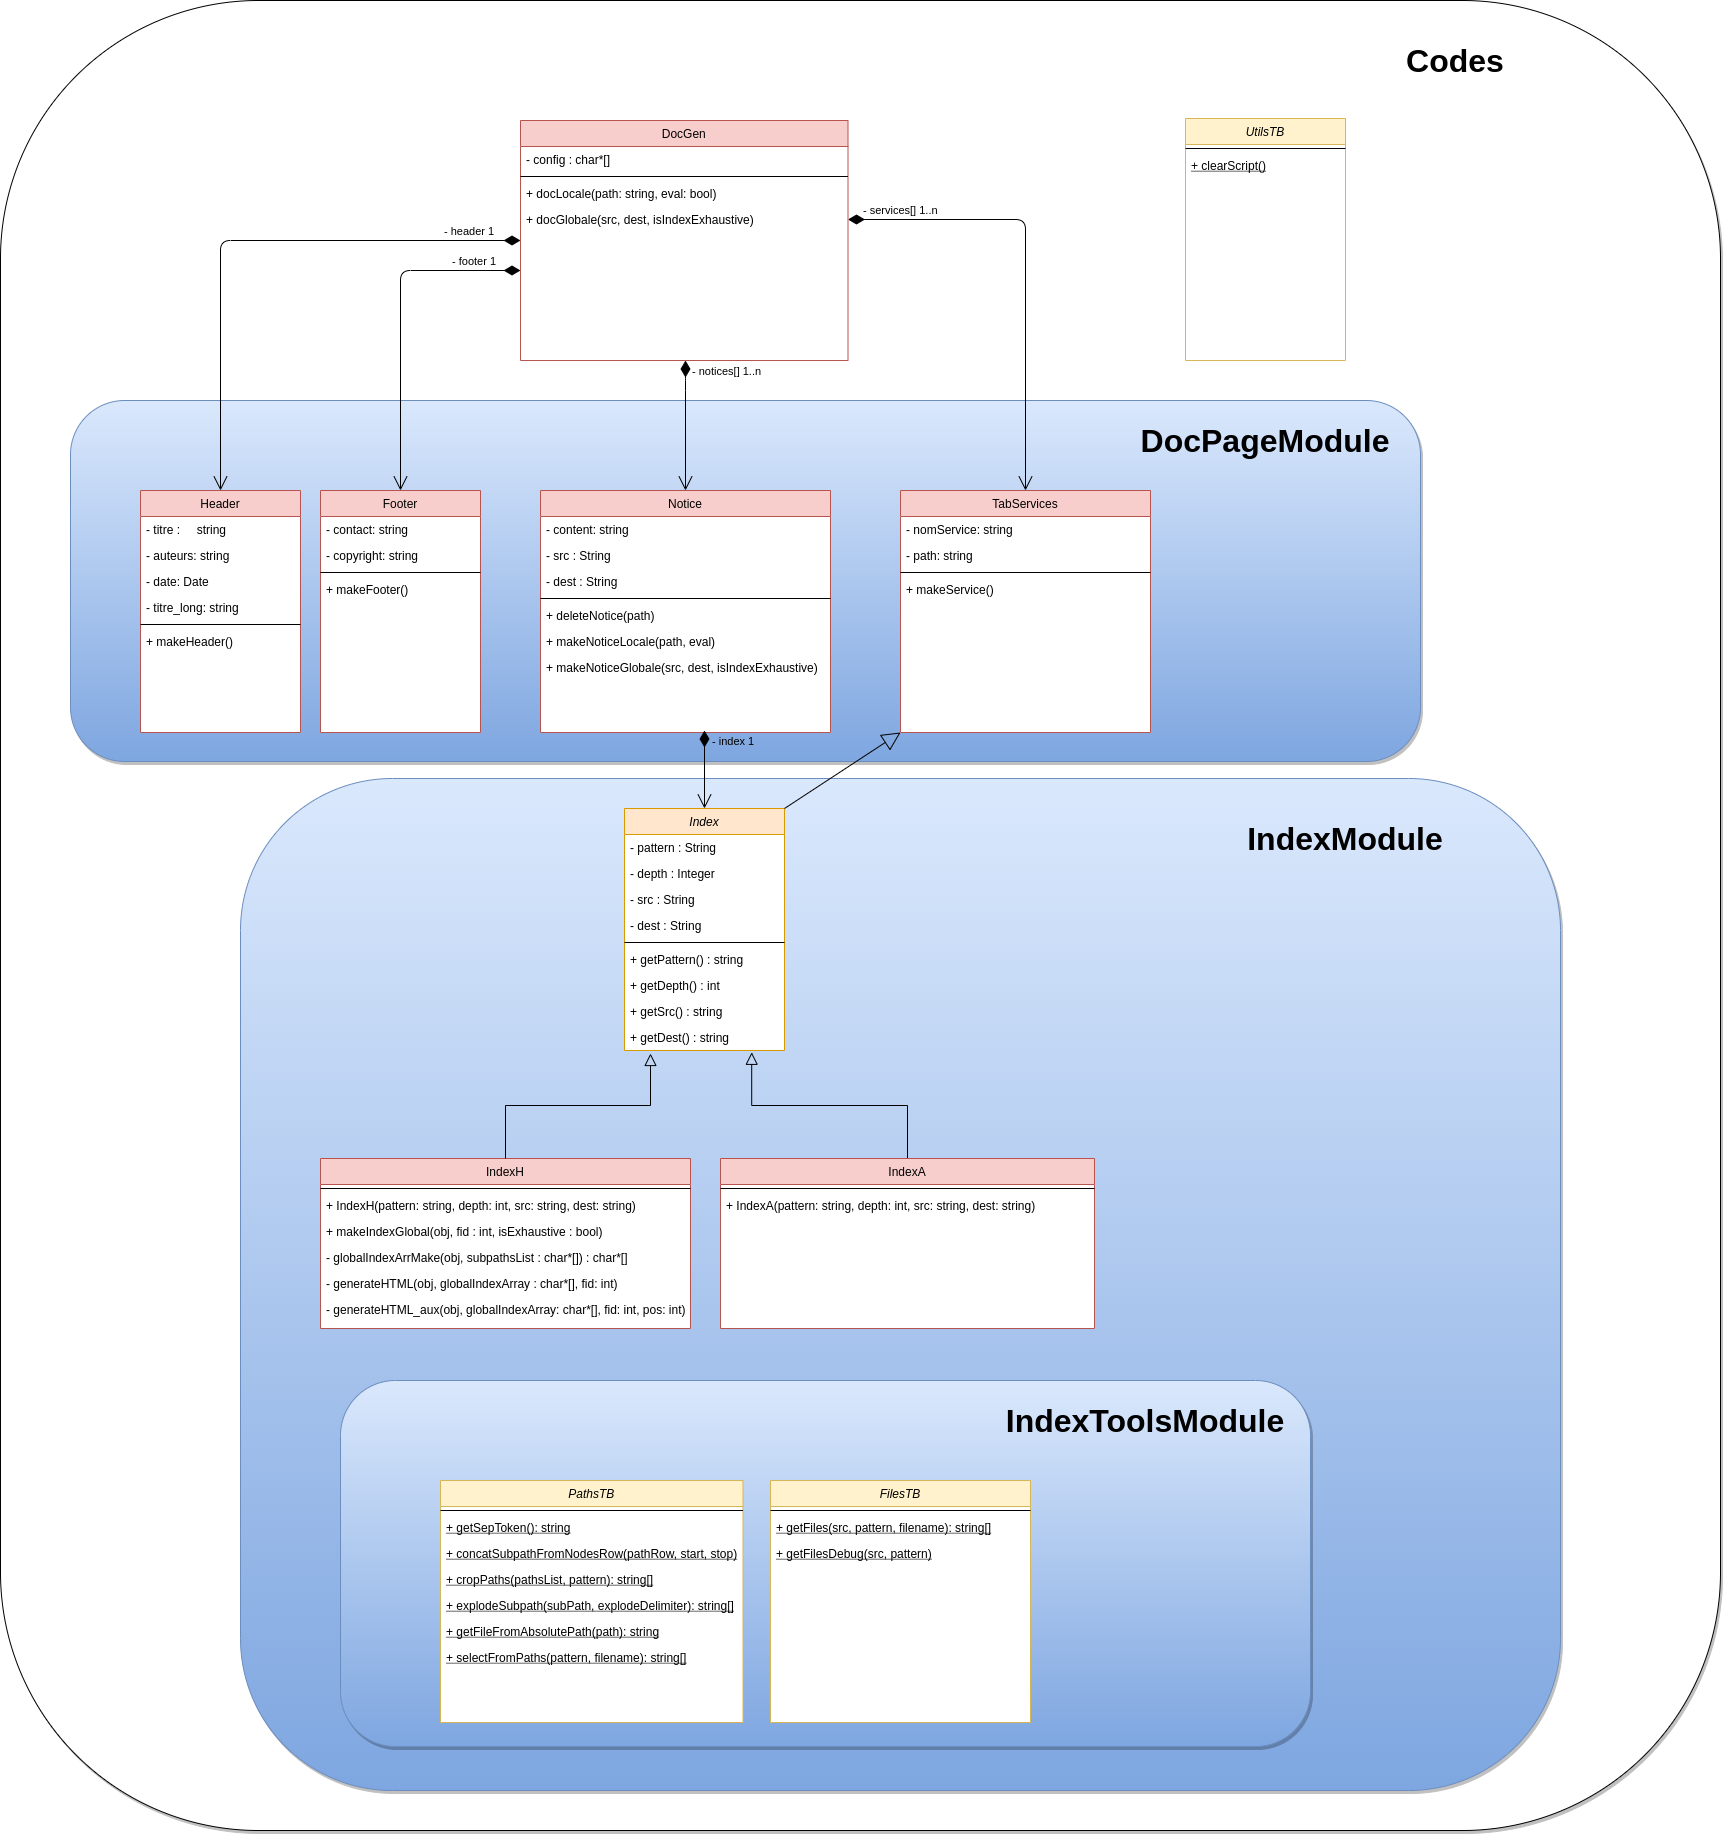
\includegraphics[scale=0.225]{../DocGen.png}
	\caption{Diagramme de classe de DocGen}
	\label{fig:indexT}
\end{figure}


%%% #################### LE HEADER  #################### %%%
\chapter{Génération du Header}


%%% #################### LES INDEX  #################### %%%
\chapter{Génération des Index}

%%  ================== INDEX HIERARCHIQUES ====================  %%
\section{Index hiérarchiques}

\subsection{Définition}
Un index hiérarchique ou arborescent est une forme d'indexation où les entrées sont contenues dans d'autres entrées, etc. reflétant ainsi la généralisation (on remonte dans l'arbre) ou la spécification (on descend dans l'arbre) des entrées les unes par rapport aux autres.\\

Ce type d'index est appelé \textit{indexT} dans le code en référance à l'anglais \textit{\textbf{T}ree Index}.\\

\begin{figure}[h!]
    \centering
    \includegraphics[scale=0.425]{images/2_specFonc/index/indexHierarchique.png}
    \caption{Exemple d'indexation hiérarchique}
    \label{fig:indexT}
\end{figure}

\newpage
\subsection{Solution 1 : Traitement d'une liste de chemins absolus}
\bigskip
\bigskip
\subsubsection{Description de l'algorithme}
\vspace{0.5cm}
\paragraph{Étape 1\\\\}
On tronque de la liste des chemins récoltés la partie correspondant à la racine où est effectué l'index et on en profite pour mettre les chemins tronqués dans un tableau de chaînes de caractères.\\

\begin{center}
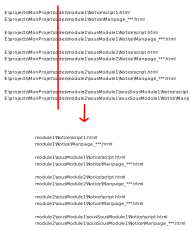
\includegraphics[scale=0.6]{images/2_specFonc/index/indexT_algo1_etape1.png}
\captionof{figure}{Suppression de la partie commune inutile}
\label{fig:indexT_algo1_etape1}
\end{center}

\newpage
\paragraph{Étape 2\\\\}
Si le paramètre \textit{isExhaustive} est à \textit{false} on supprime également de l'indexation les entrées qui ne sont pas des pages de manuel comme illustré ici:\\
\begin{center}
	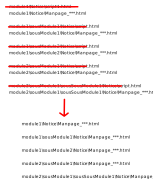
\includegraphics[scale=0.6]{images/2_specFonc/index/indexT_algo1_etape2.png}
	\captionof{figure}{Suppression des entrées qui ne sont pas des pages de manuel}
	\label{fig:indexT_algo1_etape2}
\end{center}

\newpage
\paragraph{Étape 3\\\\}
Chaque chemin absolu est ensuite traité par la méthode \textit{globalIndexArrMake(obj, subpathsList)} qui se charge d'en faire un tableau de noeuds\footnote{Une structure de donnée serait probablement plus appropriée ici...}. Les chemins absolus sont reconstitués en reconcaténant la partie tronquée à l'étape 1.
\begin{center}
	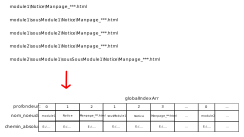
\includegraphics[scale=0.65]{images/2_specFonc/index/indexT_algo1_etape3.png}
	\captionof{figure}{Transformation des chaînes de caractères en tableaux de noeuds}
	\label{fig:indexT_algo1_etape2}
\end{center}

\newpage
\paragraph{Étape 4\\\\}

Une fois le tableau de noeud construit nous avons toutes les informations pour traduire celui-ci sous format HTML en écrivant directement dans le fichier voulu. Pour ce faire on tire profit de la récursivité dès lors qu'on s'enfonce ou qu'on remonte des profondeurs. On utilise en revanche une boucle pour le cas où on reste à la même profondeur.

Le résultat est un ensemble de listes HTML imbriquées comme illustré ici:
\begin{center}
	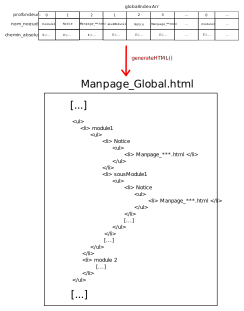
\includegraphics[scale=0.6]{images/2_specFonc/index/indexT_algo1_etape4.png}
	\captionof{figure}{Écriture du tableau de noeuds dans le fichier désigné sous format HTML}
	\label{fig:indexT_algo1_etape2}
\end{center}

\bigskip
\subsubsection{Zoom sur l'étape 3 (fonction globalIndexArrMake())}
\vspace{0.5cm}

Cette fonction, avec celle de génération du code HTML, est probablement la fonction la plus difficile à comprendre de DocGen et donc je tiens ici à offrir une description détaillée et imagée de son fonctionnement. Tout d'abord, je rappelle ici le code source: \\

\begin{lstlisting}[style=Matlab-editor, caption={Code source de la fonction de transformation de liste de chemins absolus en tableaux de noeuds},captionpos=b]
function globalIndexArray = globalIndexArrMake(obj, subpathsList)
  % Algorithm initialization %
  appendIdx = 1;
  nbSubpaths = numel(subpathsList);
  precPathRow = PathsTB.explodeSubpath(subpathsList{1}{1}, PathsTB.setgetVar);
  nbNodes = numel(precPathRow);
  for i=1:nbNodes
	nodePath = [obj.getSrc() PathsTB.setgetVar ...
	PathsTB.concatSubpathFromNodesRow(precPathRow, 1, i)];
	globalIndexArray{appendIdx} = [i, precPathRow(i), nodePath];
	appendIdx = appendIdx + 1;
  end
	
  % Global index making %
  for i=2:nbSubpaths
	currentSubpathRow = PathsTB.explodeSubpath(subpathsList{i}{1}, PathsTB.setgetVar);
	nbNodes = numel(currentSubpathRow);
	
	updatePrecPath = false;
	for j=1:nbNodes
		if j > numel(precPathRow) || ~strcmp(precPathRow(j), currentSubpathRow(j))
			updatePrecPath = true;
		end
	
		if updatePrecPath
			nodePath = [obj.getSrc() PathsTB.setgetVar ...
			PathsTB.concatSubpathFromNodesRow(currentSubpathRow, 1, j)];
			globalIndexArray{appendIdx} = [j, currentSubpathRow(j), nodePath];
			precPathRow(j) = currentSubpathRow(j);
			appendIdx = appendIdx + 1;
		end
	end
  end
end
\end{lstlisting}

\newpage
\subsubsection{Bilan}
\vspace{0.5cm}


%% ================== INDEX ALPHABETIQUES ==================== %%



%%% #################### LES NOTICES  #################### %%%
\chapter{Génération des Notices}


%%% ################# LES PAGES DE MANUEL  ################# %%%
\chapter{Génération des Pages de Manuel}

\end{document}